\documentclass[../p052main.tex]{subfiles}
\graphicspath{{\subfix{../figures/}}}

\begin{document}

\chapter{Quantum Mechanics in 3D}
\section{Particle in a 3D Box}
To begin our foray into three dimensions, let's return to the particle in a box model:
\[ V(x,y,z) = \begin{cases} 0 & 0 < x,y,z < L, \\ \infty & \text{elsewhere}. \end{cases} \]
The Hamiltonian for this potential is   
\begin{align*}
    H &= \frac{|\mbf{p}|^2}{2m} + V(x,y,z) \\
    &= -\frac{\hbar^2}{2m} \left( \frac{\partial^2}{\partial x^2} + \frac{\partial^2}{\partial y^2} + \frac{\partial^2}{\partial z^2} \right) + V(x,y,z),
\end{align*}
and the Schrödinger equation is, as usual,
\[ H \Psi = i \hbar \frac{\partial \Psi}{\partial t}, \]
where $\Psi$ is a function of time and the three spatial variables.
As before, separation of variables gives the temporal solution $f(t) = e^{-iEt / \hbar}$ and the time-independent Schrödinger equation
\[ H \psi = E \psi, \]
where $\psi$ is a function of the three spatial variables.
For our choice of potential, this becomes
\[ -\frac{\hbar^2}{2m} \left( \frac{\partial^2}{\partial x^2} + \frac{\partial^2}{\partial y^2} + \frac{\partial^2}{\partial z^2} \right) \psi = E \psi. \]
Let's do separation of variables again, this time assuming a solution of the form $\psi(x,y,z) = X(x) Y(y) Z(z)$.
Substituting and dividing by $\psi$ gives
\[ -\frac{\hbar^2}{2m} \left( \frac{1}{X} \frac{d^2 X}{d x^2} + \frac{1}{Y} \frac{d^2 Y}{d y^2} + \frac{1}{Z} \frac{d^2 Z}{d z^2} \right) = E_x + E_y + E_z, \]
where we've split the energy into three parts, one for each dimension.
For each dimension we have an equation that looks like
For each variable we have an equation that looks like
\[ -\frac{\hbar^2}{2m} \frac{d^2 X}{d x^2} = E_x X, \]
whose solution we know is
\[ X(x) = \sqrt{\frac{2}{L}} \sin \left( \frac{n_x \pi x}{L} \right), \quad E_x = \frac{n^2 \hbar^2 \pi^2}{2mL^2}, \quad n_x \in \mathbb{N}. \]
So, in all, for the three-dimensional state we have
\begin{align*}
    \psi_{n_x, n_y, n_z}(x,y,z) &= \left( \frac{2}{L} \right)^{\frac{3}{2}} \sin \left( \frac{n_x \pi x}{L} \right) \sin \left( \frac{n_y \pi y}{L} \right) \sin \left( \frac{n_z \pi z}{L} \right) \\
    E &= \left( n_x^2 + n_y^2 + n_z^2 \right) \frac{\hbar^2 \pi^2}{2mL^2}
\end{align*}
The general solution, with time dependence, involves multiplying each stationary state by a phase factor corresponding to the state's ``total energy'' $E_n = E_x + E_y + E_z$.

As an application, let's talk about Fermi energy.
Consider a macroscopic conducting cube, which we can model as a sea of valence electrons.
These electrons are ``cold'', meaning they occupy the lowest energy states they can.

Imagine a three-dimensional grid of states, each corresponding to $(n_x, n_y, n_z)$.
By the Pauli exclusion principle, each state houses up to two electrons, and the states fill from the origin outward in an eighth-circular fashion.
If we have $N$ electrons, then the maximum radius in this $n$-space is given by
\[ N = 2 \cdot \frac{1}{8} \cdot \frac{4}{3} \pi r_\textrm{max}^3 \implies r_\textrm{max} = \left( \frac{3N}{\pi} \right)^{\frac{1}{3}}, \]
and the highest energy state is
\[ E_\textrm{max} = \left( \frac{3N}{\pi} \right)^{\frac{2}{3}} \frac{\hbar^2 \pi^2}{2mL^2}. \]
This is called the Fermi energy, and it's usually written as
\[ E_F = \frac{\hbar^2}{2m} \left( 3\pi^2 \right)^{\frac{2}{3}} \left( \frac{N}{L^3} \right)^{\frac{2}{3}}. \]
Notice that the Fermi energy is only a function of the number density of electrons in the solid.

\section{Orbital Angular Momentum} %<3
In three dimensions we have many more choices for the geometry of our potentials.
One especially important class of potentials are the central potentials, which depend only on the distance $r$ from some source.
Spherical coordinates will come in handy here---we'll define $\theta$ to be the polar angle (from the $z$-axis) and $\phi$ to be the planar angle.

The time-independent Schrödinger equation for a central potential is clearly not separable in rectangular coordinates, since the potential is of the form $V(\sqrt{x^2 + y^2 + z^2})$.
But if we rewrite the equation using the Laplacian to get
\[ \left[ -\frac{\hbar^2}{2m} \nabla^2 + V(r) \right] \psi = E\psi, \]
then one could show that in spherical coordinates,
\[ \left[ -\frac{\hbar^2}{2mr^2} \left[ \frac{\partial}{\partial r} \left( r^2 \frac{\partial}{\partial r} \right) + \frac{1}{\sin \theta} \frac{\partial}{\partial \theta} \left( \sin \theta \frac{\partial}{\partial \theta} \right) + \frac{1}{\sin^2 \theta} \frac{\partial^2}{\partial \phi^2} \right] + V(r) \right] \psi = E \psi. \]
This equation might look much more complex, but it turns out to be separable!
As a first step, we'll separate the radial and angular components.

Our hint is that $\hbar$ has units of angular momentum.
Taking inspiration from Newtonian mechanics, we can get angular momentum operators in each of the three Cartesian directions:
\begin{align*}
    \hat L_x &= y \hat p_z - z \hat p_y \\
    \hat L_y &= z \hat p_x - x \hat p_z \\
    \hat L_z &= x \hat p_y - y \hat p_x
\end{align*}
Converting from rectangular to spherical coordinates,
\begin{align*}
    \hat L_x &= -\frac{\hbar}{i} \left( \sin \phi \,\frac{\partial}{\partial \theta} + \cot \theta \cos \phi \,\frac{\partial}{\partial \phi} \right) \\
    \hat L_y &= \frac{\hbar}{i} \left( \cos \phi \,\frac{\partial}{\partial \theta} - \cot \theta \sin \phi \,\frac{\partial}{\partial \phi} \right) \\
    \hat L_z &= \frac{\hbar}{i} \frac{\partial}{\partial \phi}
\end{align*}
This naturally leads to another operator,
\begin{align*}
    \hat{\mbf{L}}^2 &= \hat L_x^2 + \hat L_y^2 + \hat L_z^2 \\
    &= -\hbar^2 \left[ \frac{1}{\sin \theta} \frac{\partial}{\partial \theta} \left( \sin \theta \frac{\partial}{\partial \theta} \right) + \frac{1}{\sin^2 \theta} \frac{\partial^2}{\partial \phi^2} \right]
\end{align*}
But this is precisely what we see in the spherical time-independent Schrödinger equation!
So we can write
\[ \left[ -\frac{\hbar^2}{2mr^2} \frac{\partial}{\partial r} \left( r^2 \frac{\partial}{\partial r} \right) + \frac{\hat{\mbf{L}}^2}{2mr^2} + V(r) \right] \psi = E\psi. \]
We can see that $H$ and $\hat{\mbf{L}}^2$ commute, so they have a common set of eigenfunctions.
The eigenfunctions of $\hat{\mbf{L}}^2$ are of the form $Y(\theta, \phi)$ and the Hamiltonian only adds a radial component, so the combined eigenfunctions have the form $\psi_E (r,\theta,\phi) = R(r) Y(\theta, \phi)$.

We'll focus on the angular stuff for now.
The eigenvalue equation for $\hat{\mbf{L}}^2$ is
\begin{align*}
    -\hbar^2 \left[ \frac{1}{\sin \theta} \frac{\partial}{\partial \theta} \left( \sin \theta \frac{\partial}{\partial \theta} \right) + \frac{1}{\sin^2 \theta} \frac{\partial^2}{\partial \phi^2} \right] Y(\theta, \phi) &= L^2 Y (\theta, \phi), \\
    \intertext{but notice that we can immediately subsitute $\hat L_z$ to get}
    \left[ \frac{-\hbar^2}{\sin \theta} \frac{\partial}{\partial \theta} \left( \sin \theta \frac{\partial}{\partial \theta} \right) + \frac{\hat L_z}{\sin^2 \theta} \right] Y(\theta, \phi) &= L^2 Y (\theta, \phi).
\end{align*}
Let's take another step down the ladder.
$\hat{\mbf{L}}^2$ commutes with $\hat L_z$, and $\hat L_z$ depends only on $\phi$, so their shared eigenfunctions can be found by employing separation of variables again.
In particular, the eigenfunctions of $\hat{\mbf{L}}^2$ are $Y(\theta, \phi) = \Theta (\theta) \Phi (\phi)$, where $\Phi$ is an eigenfunction of $\hat L_z$.
So we have the eigenvalue equation
\begin{align*}
    \hat L_z \Phi(\phi) &= L_z \Phi (\phi) \\
   \left( \frac{\hbar}{i} \frac{\partial}{\partial \phi} \right) \Phi(\phi) &= L_z \Phi (\phi) \\
   \frac{d}{d\phi} \Phi(\phi) &= \frac{iL_z}{\hbar} \Phi(\phi)
\end{align*}
Now we can see that this equation has the normalized solution
\[ \Phi(\phi) = N e^{i L_z \phi / \hbar}, \qquad N = 1 / \sqrt{2\pi}. \]
Since each point in space must have a unique value of $\psi(r,\theta,\phi)$ associated with it, $\Phi$ must be periodic with period $2\pi$.
So
\begin{align*}
    Ne^{iL_z (\phi + 2\pi) / \hbar} &= Ne^{iL_z \phi / \hbar} \\
    e^{iL_z 2\pi / \hbar} &= 1
\end{align*}
Thus $L_z = m_l \hbar$, where $m_l$ is an integer.
So the $z$-component of orbital angular momentum is quantized with eigenfunctions
\[ \Phi_{m_l}(\phi) = \frac{1}{\sqrt{2\pi}} e^{im_l \phi}. \]
Note that these eigenfunctions are orthonormal and comprise a complete basis, as we'd expect.
Also note that there's nothing that makes the $z$-direction special---we could've done the same thing for the $x$- and $y$-directions and gotten the same result!
So angular momentum is quantized in all three directions, and $\lambda \hbar^2$ is an eigenvalue for $\hat{\mbf{L}}^2$.

To add in $\theta$-dependence and find $Y(\theta, \phi)$, we use the eigenvalue equation $\hat{\mbf{L}}^2 \,Y(\theta, \phi) = \lambda \hbar^2 \,Y(\theta, \phi)$ and our definition of $Y$ to get
\[ -\hbar^2 \left[ \frac{1}{\sin \theta} \frac{d}{d\theta} \left( \sin \theta \frac{d\Theta}{d\theta} \right) - \frac{m_l^2}{\sin^2 \theta} \Theta \right] = \lambda \hbar^2 \Theta. \]
We could use power series to show that $\Theta$ is a satisfactory wave function only if $\lambda = l(l + 1)$ for whole $l$ (including $l=0$), so $L^2 = l(l+1)\hbar^2$ is quantized! %<3
The associated eigenfunctions are derived from a set of polynomials called the Legendre polynomials.
In particular,
\[ \Theta_{l,m_l}(\theta) = N_{l,m_l}(\sin \theta)^{|m_l|} \frac{d^{|m_l|} P_l(\cos\theta)}{d(\cos \theta)^{|m_l|}}, \qquad P_l(u) = \frac{1}{2^l l!} \frac{d^l}{du^l} (u^2 - 1)^l. \]
Note that we must index $\Theta$ using both $l$ and $m_l$, and since $P_l$ has at most $l$ nonzero derivatives, we have the additional restriction that $m_l = 0, \pm 1, \ldots, \pm l$.

So in all we have the angular eigenfunctions
\[ Y_{l, m_l} (\theta, \phi) = \Theta_{l, m_l}(\theta) e^{im_l \phi}. \]
These are called the spherical harmonics, and they satisfy the two equations
\begin{align*}
    \hat L_z Y_{l,m_l} (\theta, \phi) &= m_l \hbar \, Y_{l,m_l} (\theta, \phi), \quad m_l = 0, \pm 1, \ldots, \pm l \\
    \hat{\mbf{L}}^2 Y_{l,m_l} (\theta, \phi) &= l(l+1)\hbar^2 \, Y_{l,m_l} (\theta, \phi), \quad l = 0, 1, \ldots
\end{align*}
The spherical harmonics are complete and orthogonal under the inner product
\[ \int_{0}^{2\pi} \int_{0}^{\pi} Y^*_{l,m_l} Y_{l,m_l} \sin\theta \,d\theta d\phi = \delta_{l,l'} \delta_{m_l,m_l'}, \]
and we normalize one by integrating over the entire unit sphere:
\[ \int_{0}^{2\pi} \int_{0}^{\pi} |Y_{l,m_l}|^2 \sin \theta \,d\theta d\phi = 1. \]
The radial portion of $\psi$ is customarily normalized separately.

Two final side notes.
Since $L = \sqrt{L^2} = \sqrt{l(l+1)}\hbar$, and $L_z = m_l \hbar$, if $l \,m_l \neq 0$ we have $|L_z| < L$, as we might expect.
We can also evaluate the commutator
\begin{align*}
    [\hat L_x, \hat L_y] &= \left[ z, \frac{\hbar}{i} \frac{\partial}{\partial z} \right] \frac{h}{i} \left( x \frac{\partial}{\partial y} - y \frac{\partial}{\partial x} \right) \\
    &= i\hbar \hat L_z
\end{align*}
to get the uncertainty relation
\[ \Delta L_x \Delta L_y \geq \frac{\hbar}{2} \left| \left< L_z \right> \right|. \]
We can write similar relations for the other two commutators.
Two components will be on the left, and the third on the right.
The point is, we have to give up our vector notion of angular momentum since it can't point in any particular direction!

\section{Hydrogenic Atoms}
We've found the angular component $Y_{l,m_l}$ of our solution to the time-independent Schrödinger equation.
Let's get into the radial component $R$!
For starters, we could use separation of variables to show that
\[ -\frac{\hbar^2}{2mr^2} \frac{d}{dr} \left( r^2 \frac{dR}{dr} \right) + \frac{l(l+1)\hbar^2}{2mr^2} R(r) + V(r) R(r) = E R(r). \]
This is true for any radial potential, but for now we'll focus on the Coulomb potential
\[ V(r) = \frac{-Ze^2}{4\pi \epsilon_0 r} \]
for an atom with $Z$ protons and one electron, all with charge $\pm e$.
We call such an atom a hydrogenic atom.
Substituting gives
\begin{align*}
    -\frac{\hbar^2}{2m} \frac{1}{r^2} \frac{d}{dr} \left( r^2 \frac{dR}{dr} \right) + \frac{l(l+1)\hbar^2}{2mr^2} R - \frac{Ze^2}{4\pi \epsilon_0} R &= E R. \\
    \intertext{We could do some product rule magic to turn this into}
    -\frac{\hbar^2}{2mr} \frac{d^2 (rR)}{dr^2} + \frac{l(l+1)\hbar^2}{2mr^2} R - \frac{Ze^2}{4\pi \epsilon_0 r} R &= ER,
    \intertext{substituting $u(r) = rR(r)$ into which gives}
    -\frac{\hbar^2}{2m} \frac{d^2u}{dr^2} + \left[ \frac{l(l+1)\hbar^2}{2mr^2} - \frac{Ze^2}{4\pi \epsilon_0 r} \right] u &= Eu.
\end{align*}
\parbox{0.6\textwidth}{
    This looks a lot like a standard one-dimensional Hamiltonian!
    We can define the effective potential
    \[ V_\textrm{eff}(r) = \frac{l(l+1)\hbar^2}{2mr^2} - \frac{Ze^2}{4\pi \epsilon_0 r}. \]
    A sketch illustrating this potential is included at right; note that the first term is secretly a form of kinetic energy, but it serves as a ``centrifugal barrier'' that prevents the wave function from approaching zero.

    \vspace{6pt}
    Moving along, let's rewrite our equation:
}\parbox{0.4\textwidth}{
    \quad\;
    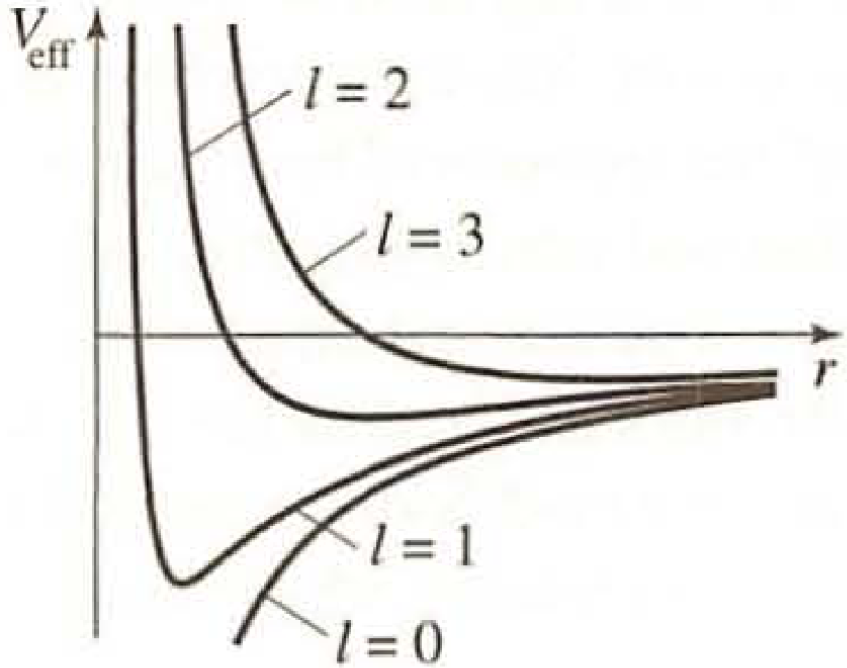
\includegraphics[width=0.35\textwidth]{hydrogenicPlot.png}
}

\[ \frac{d^2u}{dr^2} - \frac{l(l+1)u}{r^2} + 2 \frac{mZe^2}{4\pi \epsilon_0 \hbar^2} \frac{u}{r} = -\frac{2mE}{\hbar^2}u .\]
To simplify things, let's define
\[ a \equiv \frac{4\pi \epsilon_0 \hbar^2}{mZe^2} = \frac{a_0}{Z}, \quad -\frac{2mE}{\hbar^2} = \frac{1}{a^2 \lambda^2}, \]
where $a_0$ is the Bohr radius (the ``characteristic size'' of an orbital) and $\lambda$ is a dimensionless quantity.
(Notice that $E = -\hbar^2 / (2ma^2 \lambda^2)$, which resembles the particle in a box energies!)
All this gives
\[ \frac{d^2 u}{dr^2} - \frac{l(l+1)u}{r^2} + \frac{2u}{ar} - \frac{u}{a^2 \lambda^2} = 0. \]
In the limits $r \to \infty$ and $r \to 0$, the solutions to this equation are $u(r) = Be^{-Zr / \lambda a_0}$ and $u(r) = Cr^{l+1}$, respectively, where we've ignored divergent terms.
Put together, we get a reasonable guess
\[ u(r) = N r^{l+1} e^{-Zr / \lambda a_0} F(r), \]
where $F(r)$ is some power series.
Going through the motions of determining this power series gives the energies and corresponding eigenfunctions
\begin{align*}
    E_n &= -\frac{Z^2 \hbar^2}{2m a_0^2} \frac{1}{n^2} = -\frac{Z^2 e^{4} m}{2(4 \pi \epsilon_0)^2 \hbar^2} \frac{1}{n^2}, \qquad n = \lambda = l+1, l+2, \ldots \\
    R_{n,l}(r) &= \frac{u(r)}{r} = N_{n,l} r^{l} F_{n-(l+1)}(r) e^{-Zr / na_0},
\end{align*}
where $F_{n-(l+1)}$ is a Laguerre polynomial of $[n-(l+1)]$th order.
(In practice we think of $n$ as fixing the possible values of $l$.)

In summary, we have the wave function
\[ \psi_{n,l,m_l}(r,\theta,\phi) = R_{n,l} Y_{l,m_l}(\theta, \phi), \]
which is indexed by the quantum numbers
\begin{align*}
    n &= 1, 2, 3, \ldots \\
    l &= 0, 1, \ldots, n-1 \\
    m_l &= 0, \pm 1, \ldots, \pm l
\end{align*}
The wave function is normalized if the integral of $\psi^* \psi$ over all space is equal to one.
In particular,
\begin{align*}
    1 &= \int_{0}^{2\pi} \int_{0}^{\pi} \int _{0}^{\infty} (R_{n,l}^* Y_{l,m_l}^*)(R_{n,l} Y_{l,m_l}) \,r^2 \sin\theta \,dr d\theta d\phi \\
    1 &= \left[ \int _{0}^{\infty} R_{n,l}^* R_{n,l} \,r^2 \,dr \right] \left[ \int_{0}^{2\pi} \int_{0}^{\pi} Y_{l,m_l}^* Y_{l,m_l} \,\sin\theta \,d\theta d\phi \right]
\end{align*}
By convention, we normalize the radial and angular components individually.
Note that the radial probability density is $|R_{n,l}|^2 r^2$ while the angular probability density is $|Y_{l,m}|^2$.
(The probabilities get ``thinner'' as $r$ changes, but not as $\theta$ or $\phi$ change.)

All of the qualitative characteristics we determined in one dimension still hold here!
This includes node counting, but we must be careful to count the nodes in both the radial and angular components---any one individual component might not have the correct number of zeroes.
Also note that for nonzero $l$ (nonzero angular momentum), $R_{n,l}$ must go to zero at the origin.

What we've derived here is experimentally confirmed by the existence of atomic emission spectra.
When a hydrogenic atom transitions from a state with principal quantum number $n_i$ to one with $n_f$, a photon of frequency $\nu$ is emitted, where $h\nu = E_{n_i} - E_{n_f}$.
The lowest four transitions in the visible spectrum are called the Balmer series, corresponding to transitions from $n_i > 2$ to $n_f = 2$.

The energy of the atom is fully described by its principal quantum number $n$, but there are multiple eigenstates corresponding to this energy.
In particular, there is one eigenstate for each allowed $l$ and $m_l$, so the degeneracy of each energy is given by the sum
\[ \sum_{l=0}^{n-1} (2l + 1) = n^2. \]
Soon we'll introduce a fourth quantum number that brings this number up to $2n^2$.

Note that these eigenfunctions are stationary states, so they don't correspond to an electron classically ``orbiting'' a nucleus.
But there is an associated probability current!
In particular, we can show that
\begin{align*}
    \mbf{j} &= \frac{\hbar}{2mi} \left( \psi^* \nabla \psi - \psi \nabla \psi^* \right) \\
    &= \frac{\hbar m_l}{mr \sin \theta} |\psi_{n,l,m_l}(r,\theta,\phi)|^2 \,\hat\phi
\end{align*}
This is completely analogous to an electric current in a loop of wire---though the charge is moving, the amount of charge at any given point along the loop is constant over time.

\section{The Zeeman Effect}
Something interesting happens when we add a magnetic field to the scenario.
Let's first consider an analogous classical picture.
A particle with charge $q$ an mass $m$ moves in a circular orbit of radius $r$ with speed $v$.
The current $I = qv / (2\pi r)$ associated with this particle corresponds to a magnetic dipole moment of magnitude
\[ \mu = I \cdot \pi r^2 = \frac{qrv}{2}. \]
But $L = rmv$, so we can write this as $\boldsymbol\mu = (q / 2m) \mbf{L}$.
If this particle is in a magnetic field $\mbf{B} = B \hat z$, then the energy of interaction is
\[ -\boldsymbol\mu \cdot \mbf{B} = -\frac{q}{2m} \mbf{L} \cdot \mbf{B} = -\frac{qB}{2m}L_z. \]
This suggests that if we were to immerse a hydrogenic atom in an external magnetic field in the $z$-direction, then we will need to add an extra $(q_e B / 2m) \hat L_z$ term to the Hamiltonian.
So we have
\[ \hat H = \left( -\frac{\hbar^2}{2m} \nabla^2 - \frac{Ze^2}{4\pi \epsilon_0 r} \right) + \frac{q_e B}{2m} \hat L_z. \]
The eigenfunctions for the old Hamiltonian still hold here---they are eigenfunctions for $\hat L_z$, so the new term doesn't change anything.
The new eigenvalues are simply
\[ E_{n,m_l} = E_n + \frac{q_e B}{2m} m_l \hbar = E_n + \mu_B m_l B, \]
where $E_n$ are the energies without the magnetic field and $\mu_B = q_e \hbar / 2m$ is the very small ``Bohr magneton'' correction.
This breaks the degeneracy of each energy level with respect to $m_l$, which can be observed in emission lines.
A transition from $l=1$ to $l=0$, for example, would result in three very slightly different frequencies for emitted light.

If we look even more closely at the emission lines, though, an interesting phenomenon emerges.
For example, if we were to fire a beam of $l=0$ silver atoms through a magnetic field with a vertical magnitude gradient, we'd expect to see no Zeeman splitting since there's only one allowed $m_l$.
But the Stern-Gerlach experiment showed that the beam actually splits into two!
This splitting cannot be explained using the quantum mechanics we've done so far, so we're forced to introduce a new property of particles: spin.

\section{Intrinsic Spin}
Spin angular momentum $\mbf{S}$ is a completely new property of particles with no classical equivalent.
For an electron, its associated magnetic moment is
\[ \boldsymbol\mu = -g \frac{q_e}{2m} \mbf{S}, \]
where $g$ is a ``fudge factor'' introduced to provide agreement with experiment.
The total magnetic moment can be found by adding the individual moments from orbital and spin angular momentum.

We define spin in a very similar fashion to orbital angular momentum.
For one, the same commutation relations hold:
\begin{align*}
    [\hat S_x, \hat S_y] &= i\hbar \hat S_z \\
    [\hat S_y, \hat S_z] &= i\hbar \hat S_x \\
    [\hat S_z, \hat S_x] &= i\hbar \hat S_y
\end{align*}
We also have similar eigenvalue equations:
\begin{align*}
    \hat S_z \chi &= m_s \hbar \chi, \quad m_s = 0, \pm \frac{1}{2}, \ldots, \pm s \\
    \hat{\mbf{S}}^2 \chi &= s(s+1)\hbar^2 \chi, \quad s = 0, \frac{1}{2}, 1, \ldots
\end{align*}
Unlike the orbital $l$-values, which depend on the physical state of the particle, the value of $s$ is an intrinsic property of the particle that cannot be changed.
Despite this, orbital and spin angular momentum are still both angular momentum and one type may be converted to another.
Despite the fundamental difference between orbital and spin angular momentum, though, they are still both angular momentum and one type may be converted to another.

Observations indicate that $s = 1/2$ for all ``matter particles'' like electrons.
Thus these particles only have two spin eigenstates, which we'll call $\chi_+$ (``spin up'') and $\chi_-$ (``spin down'').
These eigenstates form a complete, orthonormal basis, so any spin state can be expressed as $\chi = c_+ \chi_+ + c_- \chi_-$.
We may also write this in vector notation:
\[ \chi_+ = \begin{bmatrix} 1 \\ 0 \end{bmatrix}, \quad \chi_- = \begin{bmatrix} 0 \\ 1 \end{bmatrix} \;\implies\; \chi = \begin{bmatrix} c_+ \\ c_- \end{bmatrix}. \]
In this formalism, operators are represented by matrices.
We first write down a matrix for $\hat S_z$ that yields the correct eigenvalue for each eigenstate---the easiest way to do this is to simply use the diagonal matrix
\[ \hat S_z = \frac{\hbar}{2} \begin{bmatrix} 1 & 0 \\ 0 & -1 \end{bmatrix}. \]
The other two matrix operators follow from the commutation relations:
\[ \hat S_x = \frac{\hbar}{2} \begin{bmatrix} 0 & 1 \\ 1 & 0 \end{bmatrix}, \qquad \hat S_y = \frac{\hbar}{2} \begin{bmatrix} 0 & -i \\ i & 0 \end{bmatrix}. \]
Finally, some algebra leads to
\[ \hat{\mbf{S}}^2 = \hat S_x^2 + \hat S_y^2 + \hat S_z^2 = \frac{3\hbar^2}{4} \begin{bmatrix} 1 & 0 \\ 0 & 1 \end{bmatrix}. \]
We can immediately see that
\[ [\hat S_z, \hat{\mbf{S}}^2] = 0, \]
just like with orbital angular momentum, so $\hat S_z$ and $\hat{\mbf{S}}^2$ have simultaneous eigenstates!

Consider, now, a modified version of the Stern-Gerlach experiment.
A beam of silver atoms is fired through a Stern-Gerlach device with a magnetic field in the $x$-direction; this splits the beam into two, one with $S_x = 1 / 2$ and another with $S_x = -1 / 2$.
Effectively, the device performs a measurement of $S_x$, collapsing each particle's spin state into an eigenstate.
Subsequent passes through $x$-directed magnetic fields will result in no beam splitting.
But if we were to feed, say, the $S_x = 1 / 2$ beam into a $z$-directed field, 50/50 once again splitting occurs!
We could have predicted this by simply computing the eigenvectors of the $\hat S_x$ matrix to get
\[ \chi_+^{(x)} = \frac{1}{\sqrt{2}} \begin{bmatrix} 1 \\ \pm 1 \end{bmatrix} = \frac{1}{\sqrt{2}} \chi_+ \pm \frac{1}{\sqrt{2}} \chi_-. \]
We now have a complete description of the energy eigenfunctions for a hydrogen atom:
\[ \psi_{n,l,m_l,m_s}(r,\theta,\phi) = R_{n,l}(r) Y_{l,m_l}(\theta,\phi) \chi_\pm. \]
The Zeeman eigenvalues we found earlier are also essentially correct, but there are some other subtle effects that change things slightly.
Relative motion between the electron and nucleus generates an internal magnetic field in the atom, which in turn creates a ``fine structure'' for the energy levels---even without an external field, spin-up states have slightly higher energies than spin-down ones.
The error in each from the mean looks like $E_\textrm{fs} = \boldsymbol\mu_S \cdot \mbf{B}_\textrm{int} \propto \mbf{S} \cdot \mbf{L}$.
To formalize this we may define the total angular momentum operator
\[ \hat{\mbf{J}}^2 = 2\hat{(\mbf{L} \cdot \mbf{S})} + \hat{\mbf{L}}^2 + \hat{\mbf{S}}^2; \]
this operator is quantized and has eigenvalues $J^2 = j(j+1)\hbar^2$ with $j = l \pm s$ and $m_j = 0, \pm 1, \ldots, \pm j$.
The total fine-structure energy correction turns out to depend only on $j$.

\end{document}
%<3
%<3
%<3